\section{Installare IntelliJ}
    Per svolgere gli esercizi di laboratorio, le simulazioni e l'esame userete \textbf{IntelliJ IDEA Ultimate}, non è una scelta, perciò è utile che lo usiate anche 
    quando vi esercitate a casa, inoltre imparare le varie shortcuts da tastiera vi aiuterà molto durante l'esame, sopratutto quando dovrete fare dei refactors facendovi 
    risparmiare tempo prezioso.
    Il software è normalmente a pagamento ma gli studenti hanno diritto a una licenza gratuita annuale per tutti i prodotti JetBrains, il primo step è quindi ottenere la 
    certificazione di studente.
    \subsection{Registrarsi come studente}
        È possibile registrarsi in due modi, il primo consiste nell'usare l'indirizzo email di istituto ed è quello preferibile, mentre il secondo consiste nell'inviare il certificato
        di iscrizione in inglese.
        \begin{warningbox}
            Il secondo metodo è più lungo, richiede circa una settimana perché il certificato deve essere verificato da un essere umano, ma è talvolta necessario, nel caso 
            in cui il vostro indirizzo email non venga riconosciuto.
        \end{warningbox}
        Il mio consiglio è quello di provare a registrarvi con la mail e nel caso non venisse accettata, procedere con l'invio del certificato. Indipendentemente dal metodo scelto 
        recatevi al seguente link \url{https://www.jetbrains.com/shop/eform/students}
        
        \subsubsection{Email di istituto}
            Compilate il form, prestando attenzione ad inserire l'indirizzo email nel formato 
            \textbf{nome.cognome@studenti.unitn.it}.
            \begin{figure}[H]
                \centering
                \graphicspath{{src/capitoli/04/img/}}
                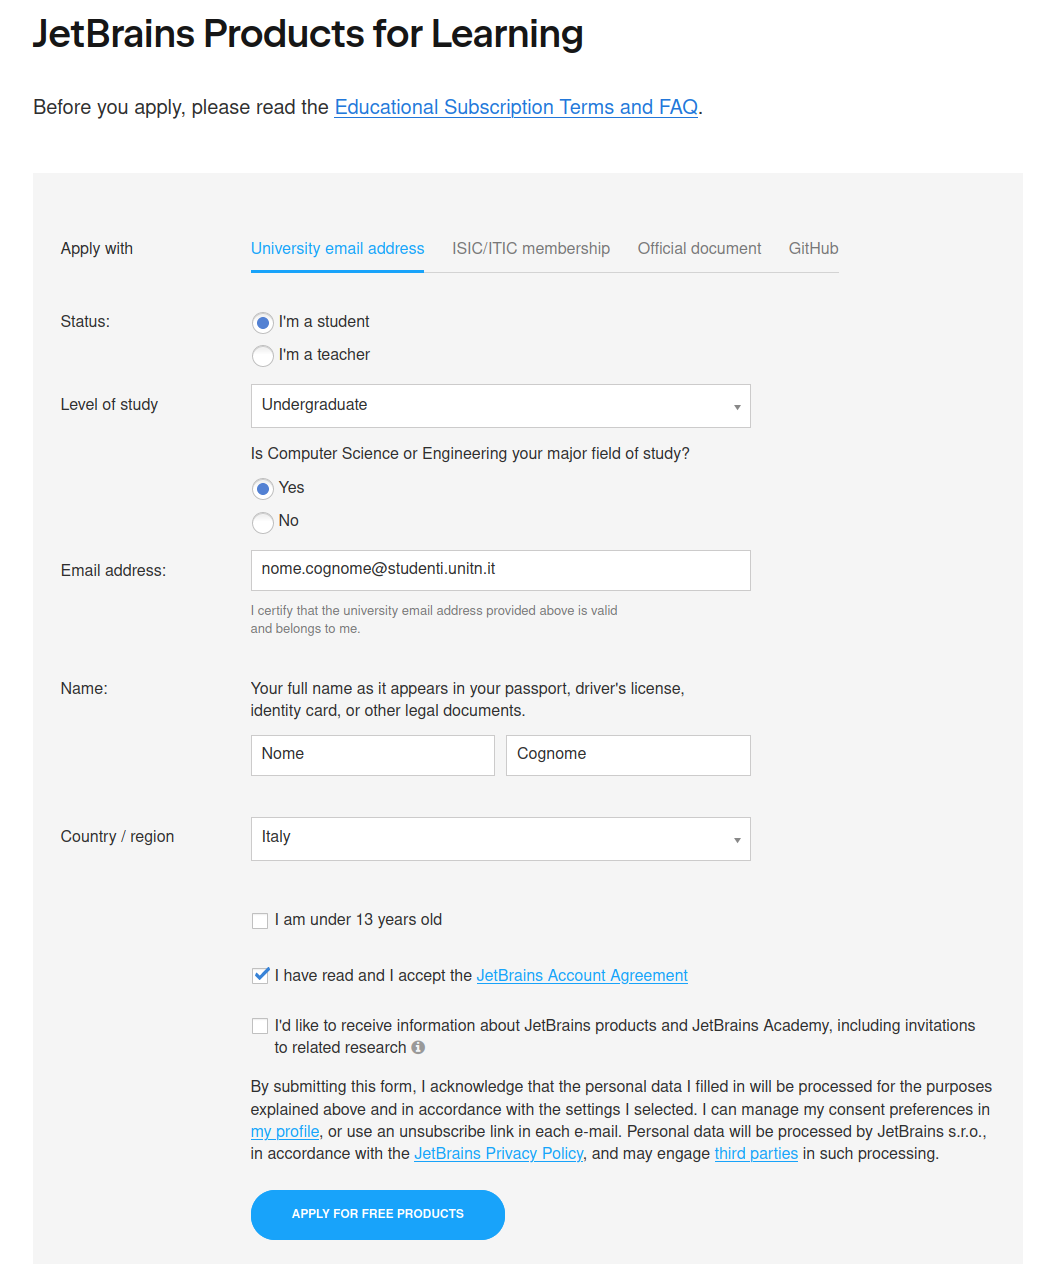
\includegraphics[width=1\textwidth]{form-studente-email.png}
                \caption{Form per la richiesta della licenza per studenti con email}
                \label{fig:Form per la richiesta della licenza per studenti con email}
            \end{figure}

            Una volta cliccato il bottone "Apply for free products" bisognerà completare il processo di certificazione aprendo il link ricevuto tramite email e completando 
            la creazione dell'account.
        
        \subsubsection{Certificato di iscrizione}
            Questa procedura richiede più passaggi, il primo dei quali è ottenere il certificato di iscrizione, andate su esse3, poi \textbf{Menù $\rightarrow$ Segreteria $\rightarrow$ My certificati} e in fine 
            cliccate su \textbf{Iscrizione con anni accademici (versione inglese)}. Scaricato il certificato tornate sulla pagina di JetBrains e selezionate apply with Official document, 
            compilate il form con i vostri dati, caricate il certificato e poi cliccate il bottone "Apply for free products".
            \begin{figure}[H]
                \centering
                \graphicspath{{src/capitoli/04/img/}}
                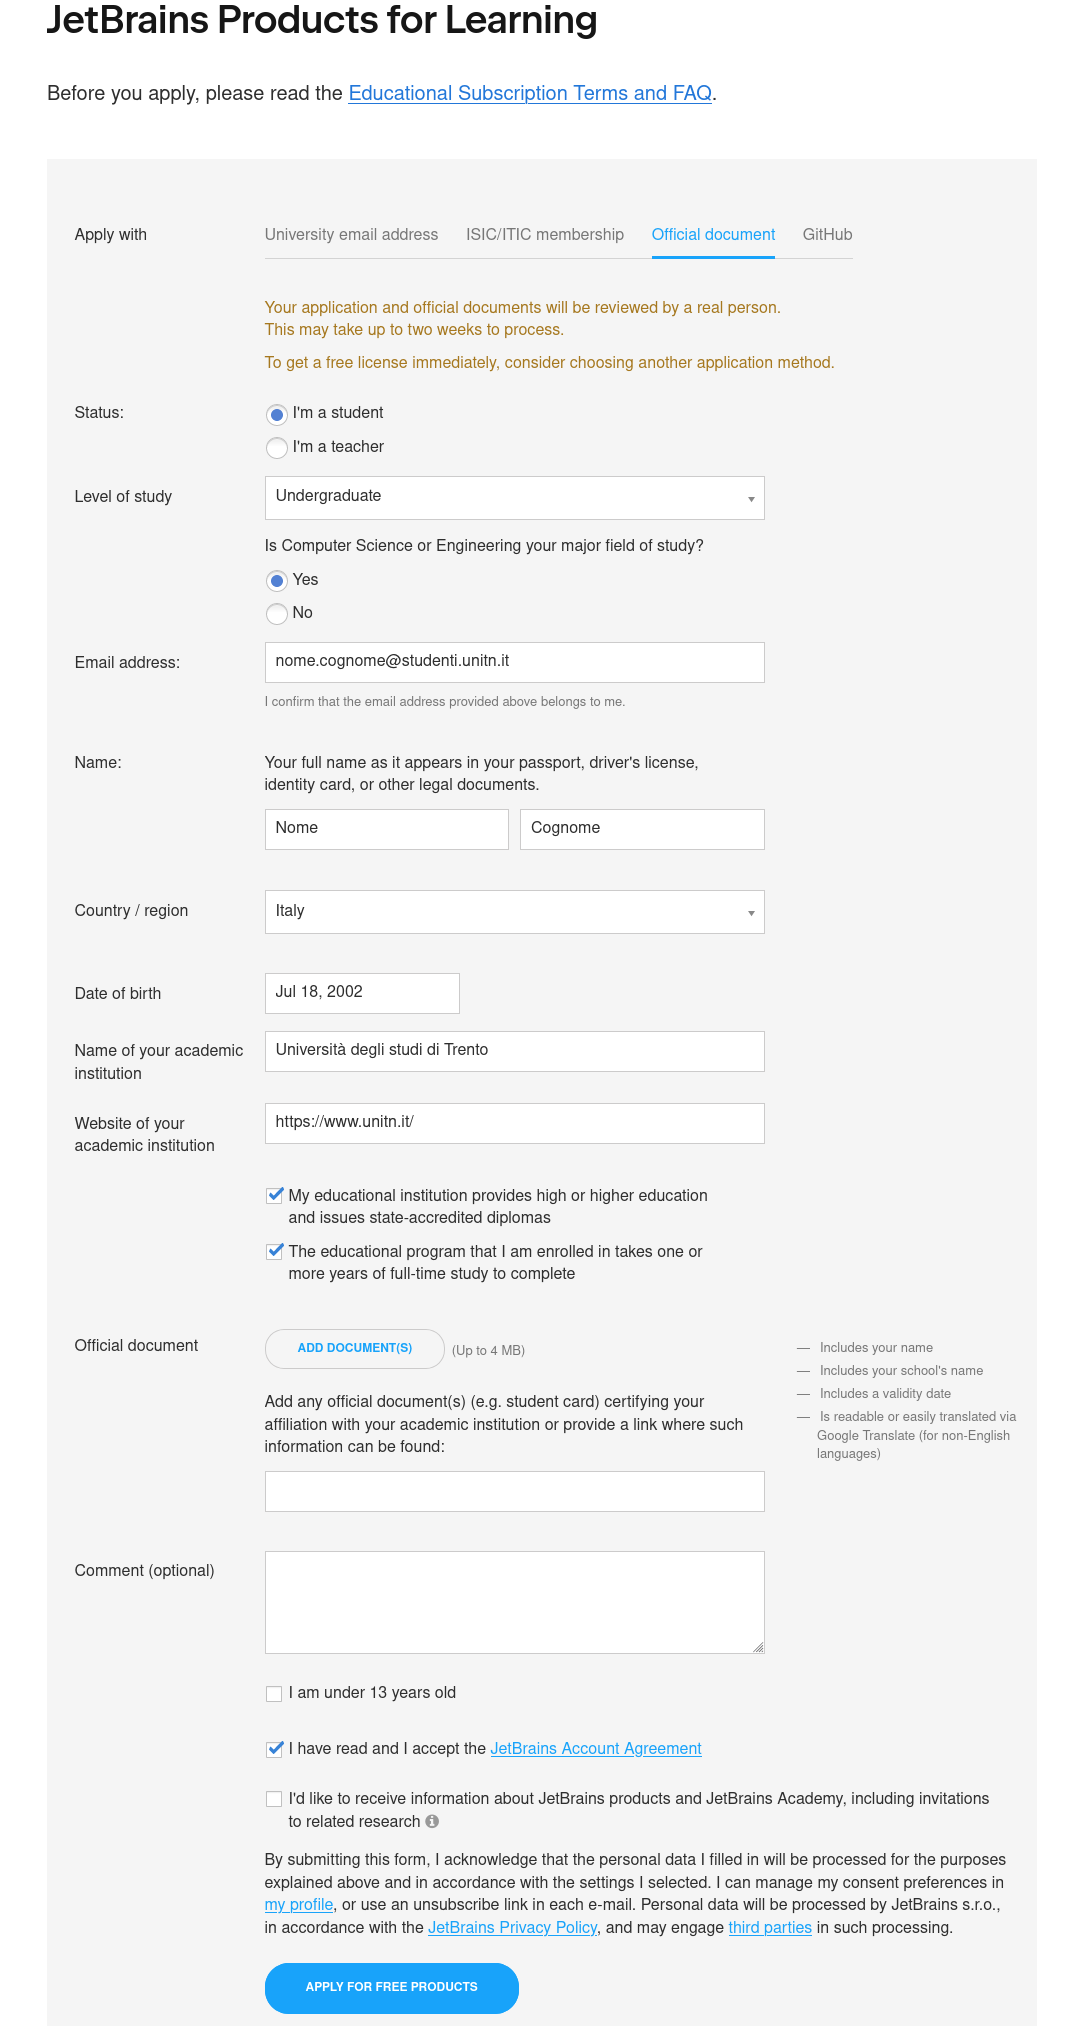
\includegraphics[width=0.7\textwidth]{form-studente-cert.png}
                \caption{Form per la richiesta della licenza per studenti con certificato}
                \label{fig:Form per la richiesta della licenza per studenti con certificato}
            \end{figure}
            Adesso dovete solo aspettare la mail di conferma per completare la creazione dell'account, solitamente richiede una settimana o più quindi abbiate pazienza.
    
    \subsection{Installare il ToolBox}
        Il modo più semplice per installare e mantenere aggiornati i prodotti JetBrains è utilizzare il ToolBox, un programma che consente di scaricare e mantenere aggiornati 
        tutti gli IDE di JetBrains, recatevi all'indirizzo \url{https://www.jetbrains.com/toolbox-app/}

        \subsubsection{Linux}
            scaricate il file .tar.gz, apritelo ed entrate nell'unica cartella presente, estraete il file e recatevi nella cartella in cui lo avete estratto. cliccate due volte col tasto 
            sinistro sul file chiamato jetbrains-toolbox e aspettate che vi si apra la seguente finestra (potrebbe richiedere una decina di secondi)
            \begin{warningbox}
                Nel caso in cui la finestra non compaia (dopo aver aspettato un intervallo di tempo ragionevole), o l'abbiate chiusa per errore, 
                basterà andare nel \textbf{system tray} (barra delle notifiche), e cercare l'icona di una scatola rosa e nera. Per esempio in Ubuntu:
                \begin{figure}[H]
                    \centering
                    \graphicspath{{src/capitoli/04/img/}}
                    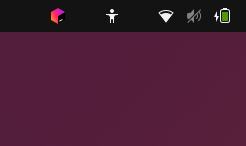
\includegraphics[width=0.5\textwidth]{barra-toolbox.png}
                    \caption{Icona del toolbox nel system tray di Gnome}
                    \label{fig:Icona del toolbox nel system tray di Gnome}
                \end{figure}
                se non fosse presente nel system tray, cercate nel menù delle applicazioni del vostro ambiente desktop, nel raro caso in cui non sia presente 
                nemmeno li, allora probabilmente vi manca \textbf{libfuse}, vi invito a \textbf{cercare su Google il nome della vostra distribuzione seguito dalla versione 
                e dalla frase "jetbrains toolbox won't start"}, sicuramente troverete una guida che saprà aiutarvi.
            \end{warningbox}            

        \subsubsection{Windows}
            scaricate il file .exe, apritelo e cliccate sul tasto \textbf{Install},
            \begin{figure}[H]
                \centering
                \graphicspath{{src/capitoli/04/img/}}
                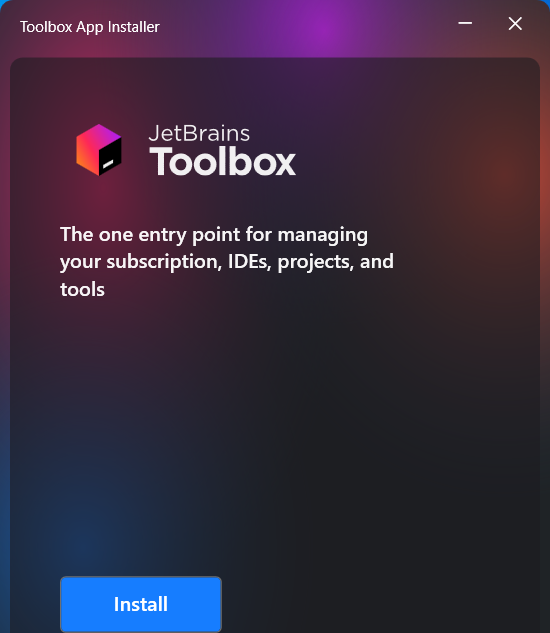
\includegraphics[width=0.4\textwidth]{toolbox-windows.png}
                \caption{Installer del toolbox su Windows}
                \label{fig:Installer del toolbox su Windows}
            \end{figure}
            aspettate che finisca e che vi si apra la finestra del toolbox, \textbf{nel caso non la troviate} 
            controllate la system tray
            \begin{figure}[H]
                \centering
                \graphicspath{{src/capitoli/04/img/}}
                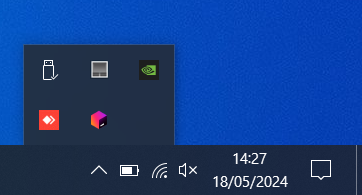
\includegraphics[width=0.5\textwidth]{toolbox-tray-windows.png}
                \caption{Icona del toolbox nel system tray di Windows}
                \label{fig:Icona del toolbox nel system tray di Windows}
            \end{figure}

        \subsubsection{MacOS}
            scaricate il file .dmg \textbf{prestando attenzione all'architettura del vostro Mac: macOS Intel per i processori x64 e macOS Apple 
            Silicon per i processori della serie M} macOS Intel per i processori x64 apritelo e seguite le istruzioni trascinando l'applicazioni 
            all'interno della cartella Applications, dopodiché avviatela cercandola nel menù delle applicazioni.\clearpage

    \subsection{Utilizzare il ToolBox}
        Quando vi si sarà presentata la seguente finestra:
        \begin{figure}[H]
            \centering
            \graphicspath{{src/capitoli/04/img/}}
            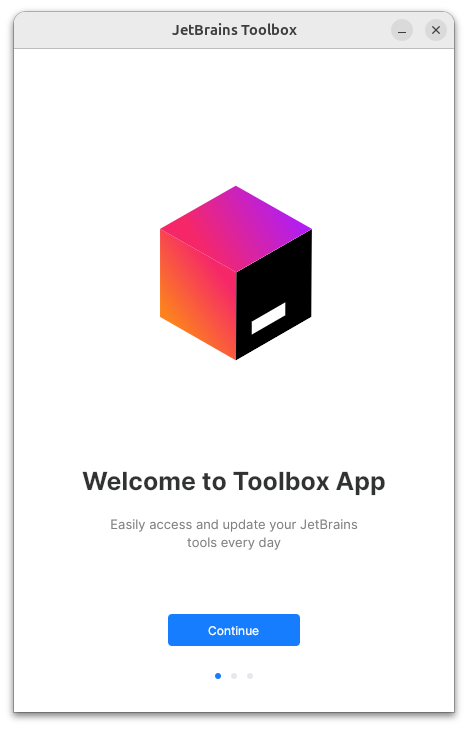
\includegraphics[width=0.5\textwidth]{toolbox-primo-avvio.png}
            \caption{Primo avvio del toolbox}
            \label{fig:Primo avvio del toolbox}
        \end{figure}
        cliccate su \textbf{Continue $\rightarrow$ Accept License Agreement $\rightarrow$ Get Started}.
        
        dopodiché cliccate nella rotella in alto a destra e poi su \textbf{Log in}
        \begin{figure}[H]
            \centering
            \graphicspath{{src/capitoli/04/img/}}
            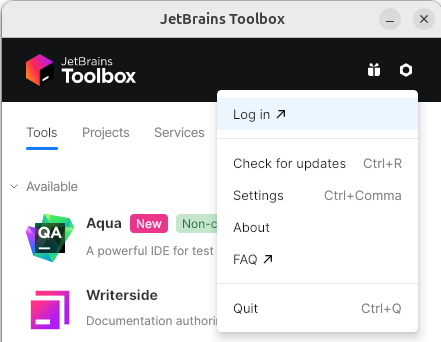
\includegraphics[width=0.4\textwidth]{toolbox-login.png}
            \caption{Menù per effettuare il login sul toolbox}
            \label{fig:Menù per effettuare il login sul toolbox}
        \end{figure}

        vi si aprirà il browser di default sulla pagina di login di JetBrains, inserite le credenziali del vostro account, sul quale avete 
        attiva la licenza da studenti
        \begin{figure}[H]
            \centering
            \graphicspath{{src/capitoli/04/img/}}
            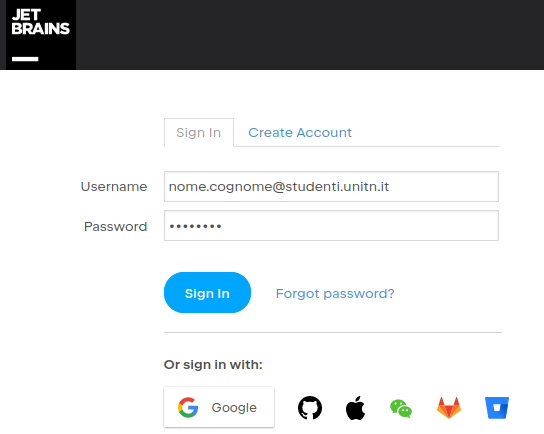
\includegraphics[width=0.5\textwidth]{toolbox-login-web.png}
            \caption{Pagina web di login al vostro account}
            \label{fig:Pagina web di login al vostro account}
        \end{figure}
        e poi cliccate su \textbf{Sign In}. Vi comparirà una finestra del browser che vi chiederà il consenso per aprire il toolbox, \textbf{acconsentite}.
        